\documentclass[11pt,a4paper]{article}
\usepackage[english]{babel}					% Use english
\usepackage[utf8]{inputenc}					% Caracteres UTF-8
\usepackage{graphicx}						% Imagenes
\usepackage[hidelinks]{hyperref}			% Poner enlaces sin marcarlos en rojo
\usepackage{fancyhdr}						% Modificar encabezados y pies de pagina
\usepackage{float}							% Insertar figuras
\usepackage[textwidth=390pt]{geometry}		% Anchura de la pagina
\usepackage[nottoc]{tocbibind}				% Referencias (no incluir num pagina indice en Indice)
\usepackage{enumitem}						% Permitir enumerate con distintos simbolos
\usepackage[T1]{fontenc}					% Usar textsc en sections
\usepackage{amsmath}						% Símbolos matemáticos
\usepackage{amsfonts}
\usepackage{subcaption}

% Comando para poner el nombre de la asignatura
\newcommand{\subject}{Numerical Linear Algebra}
\newcommand{\autor}{Vladislav Nikolov Vasilev}
\newcommand{\titulo}{Project 2}
\newcommand{\subtitulo}{SVD Applications}
\newcommand{\masters}{Master in Fundamental Principles of Data Science}


% Configuracion de encabezados y pies de pagina
\pagestyle{fancy}
\lhead{\autor{}}
\rhead{\subject{}}
\lfoot{\masters}
\cfoot{}
\rfoot{\thepage}
\renewcommand{\headrulewidth}{0.4pt}		% Linea cabeza de pagina
\renewcommand{\footrulewidth}{0.4pt}		% Linea pie de pagina

\begin{document}
\pagenumbering{gobble}

% Title page
\begin{titlepage}
  \begin{minipage}{\textwidth}
    \centering
    
\includegraphics[scale=0.25]{img/ub-logo}\\[2cm]
    
    \textsc{\Large \subject\\[0.5cm]}
    \textsc{\uppercase\expandafter{\masters}}\\[1.5cm]
    
    \noindent\rule[-1ex]{\textwidth}{1pt}\\[1.5ex]
    \textsc{{\Huge \titulo\\[0.5ex]}}
    \textsc{{\Large \subtitulo\\}}
    \noindent\rule[-1ex]{\textwidth}{2pt}\\[3.5ex]
  \end{minipage}
  
  \vspace{2cm}
  
  \begin{minipage}{\textwidth}
    \centering
    
    
\includegraphics[scale=0.4]{img/ub-ds-logo}
    \vspace{2cm}
    
    \textbf{Author}\\ {\autor{}}\\[2.5ex]
    \textsc{Faculty of Mathematics and Computer Science}\\
    \vspace{1em}
    \textsc{Academic year 2021-2022}
  \end{minipage}
\end{titlepage}

\pagenumbering{arabic}
\tableofcontents
\thispagestyle{empty}				% No usar estilo en la pagina de indice

\newpage

\setlength{\parskip}{1em}
\setlength{\parindent}{0pt}

\section{Introduction}

The goal of this project is to discuss three common applications of the Singular Value
Decomposition (SVD). First, let's briefly review what the SVD is.

Given a rectangular matrix $A \in \mathbb{R}^{m \times n}$ with $m \geq n$, we can express
it as

\[
  A = U \Sigma V^T
\]

where $U \in \mathbb{R}^{m \times m}$ and $V \in \mathbb{R}^{n \times n}$ are two orthogonal basis
and $\Sigma \in \mathbb{R}^{m \times n}$ is a matrix that can be divided in the diagonal block
$\Sigma\left[1:n, 1:n\right]$ with the singular values the singular values $\sigma_i$ in the diagonal
and the zero block $\Sigma\left[(m-n):m, 1:n\right]$. The singular values are ordered such that
$\sigma_1 \geq \sigma_2 \geq \dots \geq \sigma_n \geq 0$. Since $U$ and $V$ are orthogonal, we have
that $U^{-1} = U^T$ and $V^{-1} = V^T$.

There are some cases in which we can also compute a reduced version of the SVD, which is faster and
reduces the amount of memory needed to store the matrices. This can be particularly useful in scenarios
where the matrix $A$ is rank deficient.

Let $A \in \mathbb{R}^{m \times n}$ be a rectangular matrix with $rank(A) = r$, where $r < n$. For this
case, the reduced SVD can be computed as

\begin{equation}
  \label{eq:reduced-svd}
  A = U_r \Sigma_r V_r^T
\end{equation}


where $U_r \in \mathbb{R}^{m \times r}$ and $V_r^T \in \mathbb{R}^{r \times r}$ are the orthogonal
basis and $\Sigma \in \mathbb{R}^{r \times r}$ is the diagonal matrix containing the nonzero
singular values.

There are many applications of the SVD, but in this project we are going to focus on three of them:
solving the Least Squares Problem, image compression and Principal Component Analysis.

\section{Least Squares Problem}

The first application that we are going to address is the Least Squares Problem (LSP). Recall that
in this problem we have a matrix $A \in \mathbb{R}^{m \times n}$ with $m \geq n$ and a vector
$b \in \mathbb{R}^m$. Our goal is to find a vector $x \in \mathbb{R}^n$ such that $Ax$ is as close
to $b$ as possible. This can be expressed as a minimization problem, in which we have

\begin{equation}
  \label{eq:lsp}
  \min ||Ax-b||_2
\end{equation}

There are many ways in which we can solve this problem: using iterative methods, normal equations,
QR factorization or SVD, among many others. In this case, we are going to focus on the SVD method,
which is also very appropriate for the rank deficient case.

Consider the reduced version of the SVD seen in expression \eqref{eq:reduced-svd}. We can use it to
compute the \emph{Moore-Penrose inverse} (also called \emph{pseudo-inverse}) of our matrix $A$ as

\[
  A^+ = V_r \Sigma_r^{-1} U_r^T
\]

with $A^+ \in \mathbb{R}^{n \times m}$. Thus, we can express the minimization problem \eqref{eq:lsp}
as follows:

\[
  x = A^+ b
\]

The solution obtained with this method is well-conditioned provided that the smallest nonzero
singular value of $A$ is not too small.

To solve the LSP problem, we have created a script called \texttt{lsp.py} which contains a function
called \texttt{solve\_lsp\_svd}. This function computes the reduced SVD of an input matrix $A$,
computes the pseudo-inverse and multiplies it by the $b$ vector to get the value of $x$.
For the computation of the SVD we have used the function \texttt{numpy.linalg.svd}.
To get the rank of the matrix we have chosen the singular values greater than a certain tolerance,
which can be fixed or is computed as \texttt{Numpy} does when computing the rank of a matrix
(see implementation for further details and reference).

Let's now apply this method to some problems and see how it performs compared to another method:
the QR factorization. The before mentioned script also contains a function called
\texttt{solve\_lsp\_qr\_full\_rank}, which is used for the full rank problem, and another
one called \texttt{solve\_lsp\_qr\_rank\_deficient}, which uses the QR factorization with pivoting
to solve the rank deficient case.

\subsection{Polynomial fitting}

In this problem we are given a set of points $x$ and their values $b$. We are going to try to
approximate the values using polynomials of different degrees. To do that, we are going to use
the SVD approach both with a fixed tolerance of $10^{-10}$ and an adaptive one based on \texttt{Numpy}'s
tolerance for the computation of the rank of a matrix and the QR factorization for the full rank problem.
Once we have the projection vector $x$, we are going to compute the error of the approximation using the
$l2$ norm to see how good the it is and to compare the different methods.

\begin{figure}[H]
  \centering
  \begin{subfigure}[t]{.5\textwidth}
    \centering
    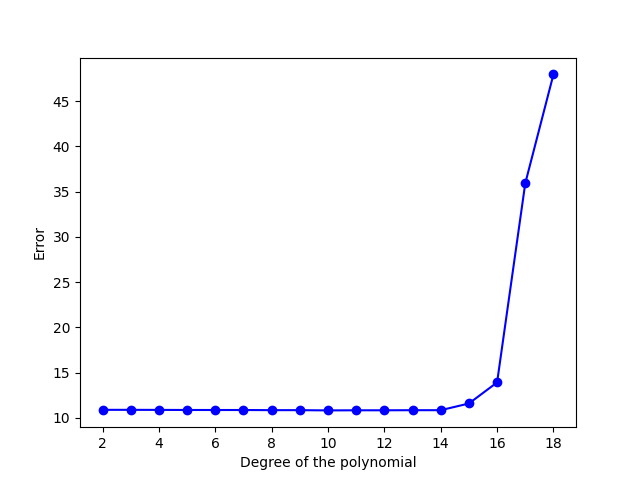
\includegraphics[scale=0.4]{img/lsp_svd_adaptive_tol}
    \caption{SVD with adaptive tolerance.}
    \label{fig:lsp-svd-adaptive-tol}
  \end{subfigure}%
  \begin{subfigure}[t]{.5\textwidth}
    \centering
    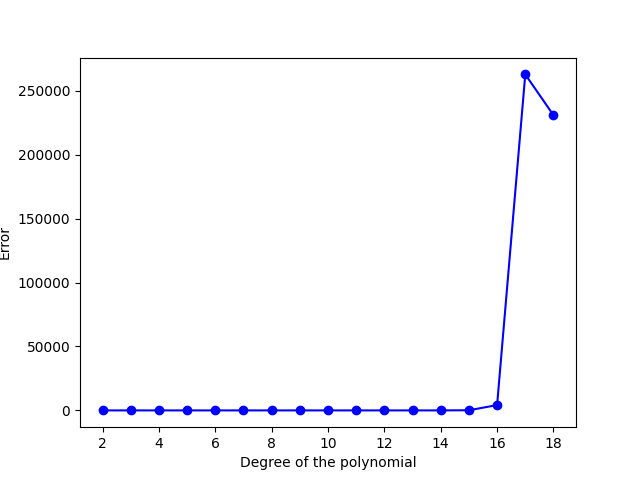
\includegraphics[scale=0.4]{img/lsp_svd_fix_tol}
    \caption{SVD with fixed tolerance.}
    \label{fig:lsp-svd-fix-tol}
  \end{subfigure}
  \begin{subfigure}[t]{.5\textwidth}
    \centering
    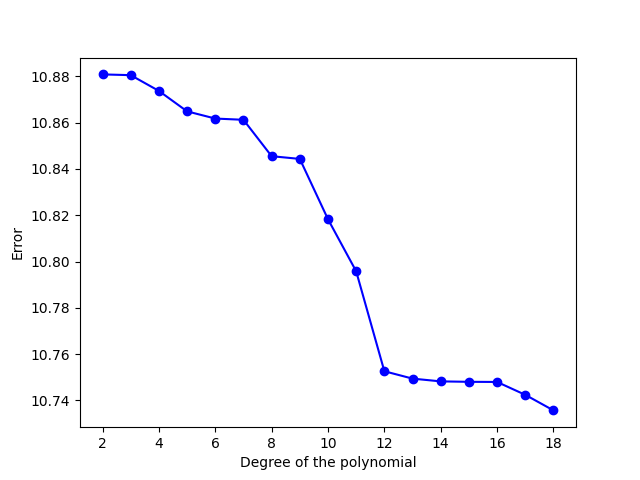
\includegraphics[scale=0.4]{img/lsp_qr}
    \caption{QR factorization without pivoting.}
    \label{fig:lsp-qr}
  \end{subfigure}
  \caption{Comparison of the approximation's error for different methods as the degree of
  the polynomial increases.}
  \label{fig:lsp-polynomial}
\end{figure}

As we can see in figure \ref{fig:lsp-polynomial}, all of the methods yield a solution which 
has approximately the same error up until polynomials of degree 13. After that point, the matrix
$A$ starts to become close to rank deficient. This has a huge impact on the SVD with fixed tolerance
because it doesn't take into account the magnitude of the singular values when discarding the less
significant ones. Therefore, the problem is treated as a full rank one, and the problem becomes
ill-conditioned because the smallest singular values are too small.

In the case of the SVD with adaptive tolerance, we can see that the error starts
increasing even when adapting the tolerance to the magnitude of the singular values so that the
problem is not treated as a full rank one. However, the error is not as large as in the previous
case.

Finally, we can see that the QR factorization without pivoting outperforms the rest of
the methods for large polynomials. It yields results with the lowest errors, and even the error seems
to decrease as the degree of the polynomial increases.

\subsection{The rank deficient LSP}

For this case, we are going to study a problem in which we have a matrix $A \in \mathbb{R}^{15 \times 11}$.
However, we have that $rank(A) = 10$ since the first two columns are exactly the same. Therefore, since
$r < n$, the matrix $A$ is going to be rank deficient.

For this problem we have used two methods: the reduced SVD with adaptive tolerance and the QR
factorization with pivoting since we cannot apply QR factorization directly to the matrix $A$.

Once again, we have solved the system and we have computed the error of the approximation using the $l2$
norm. In this case, both methods have produced approximately the same error, which is around $1.1496$.

As we can see, both method allow us to solve the problem with some small error. However, the method
based on the reduced SVD is much simpler and straightforward than the one using the QR factorization
with pivoting. Therefore, for this problem we could have used the simplest one and still get a good
result.

\section{Image compression}

\section{Principal Component Analysis}

\subsection{Example problem}

\subsection{Genes problem}

\newpage

\begin{thebibliography}{5}

\bibitem{nombre-referencia}
Texto referencia
\\\url{https://url.referencia.com}

\end{thebibliography}

\end{document}

